% Extra bottom / left (légende en bas à gauche)
\documentclass[tikz,border={30pt 28pt 60pt 30pt}]{standalone}
\usepackage{amsmath,amssymb}
\usepackage{tikz}
\usetikzlibrary{arrows.meta,positioning,fit,calc,shapes.geometric,backgrounds}

\begin{document}

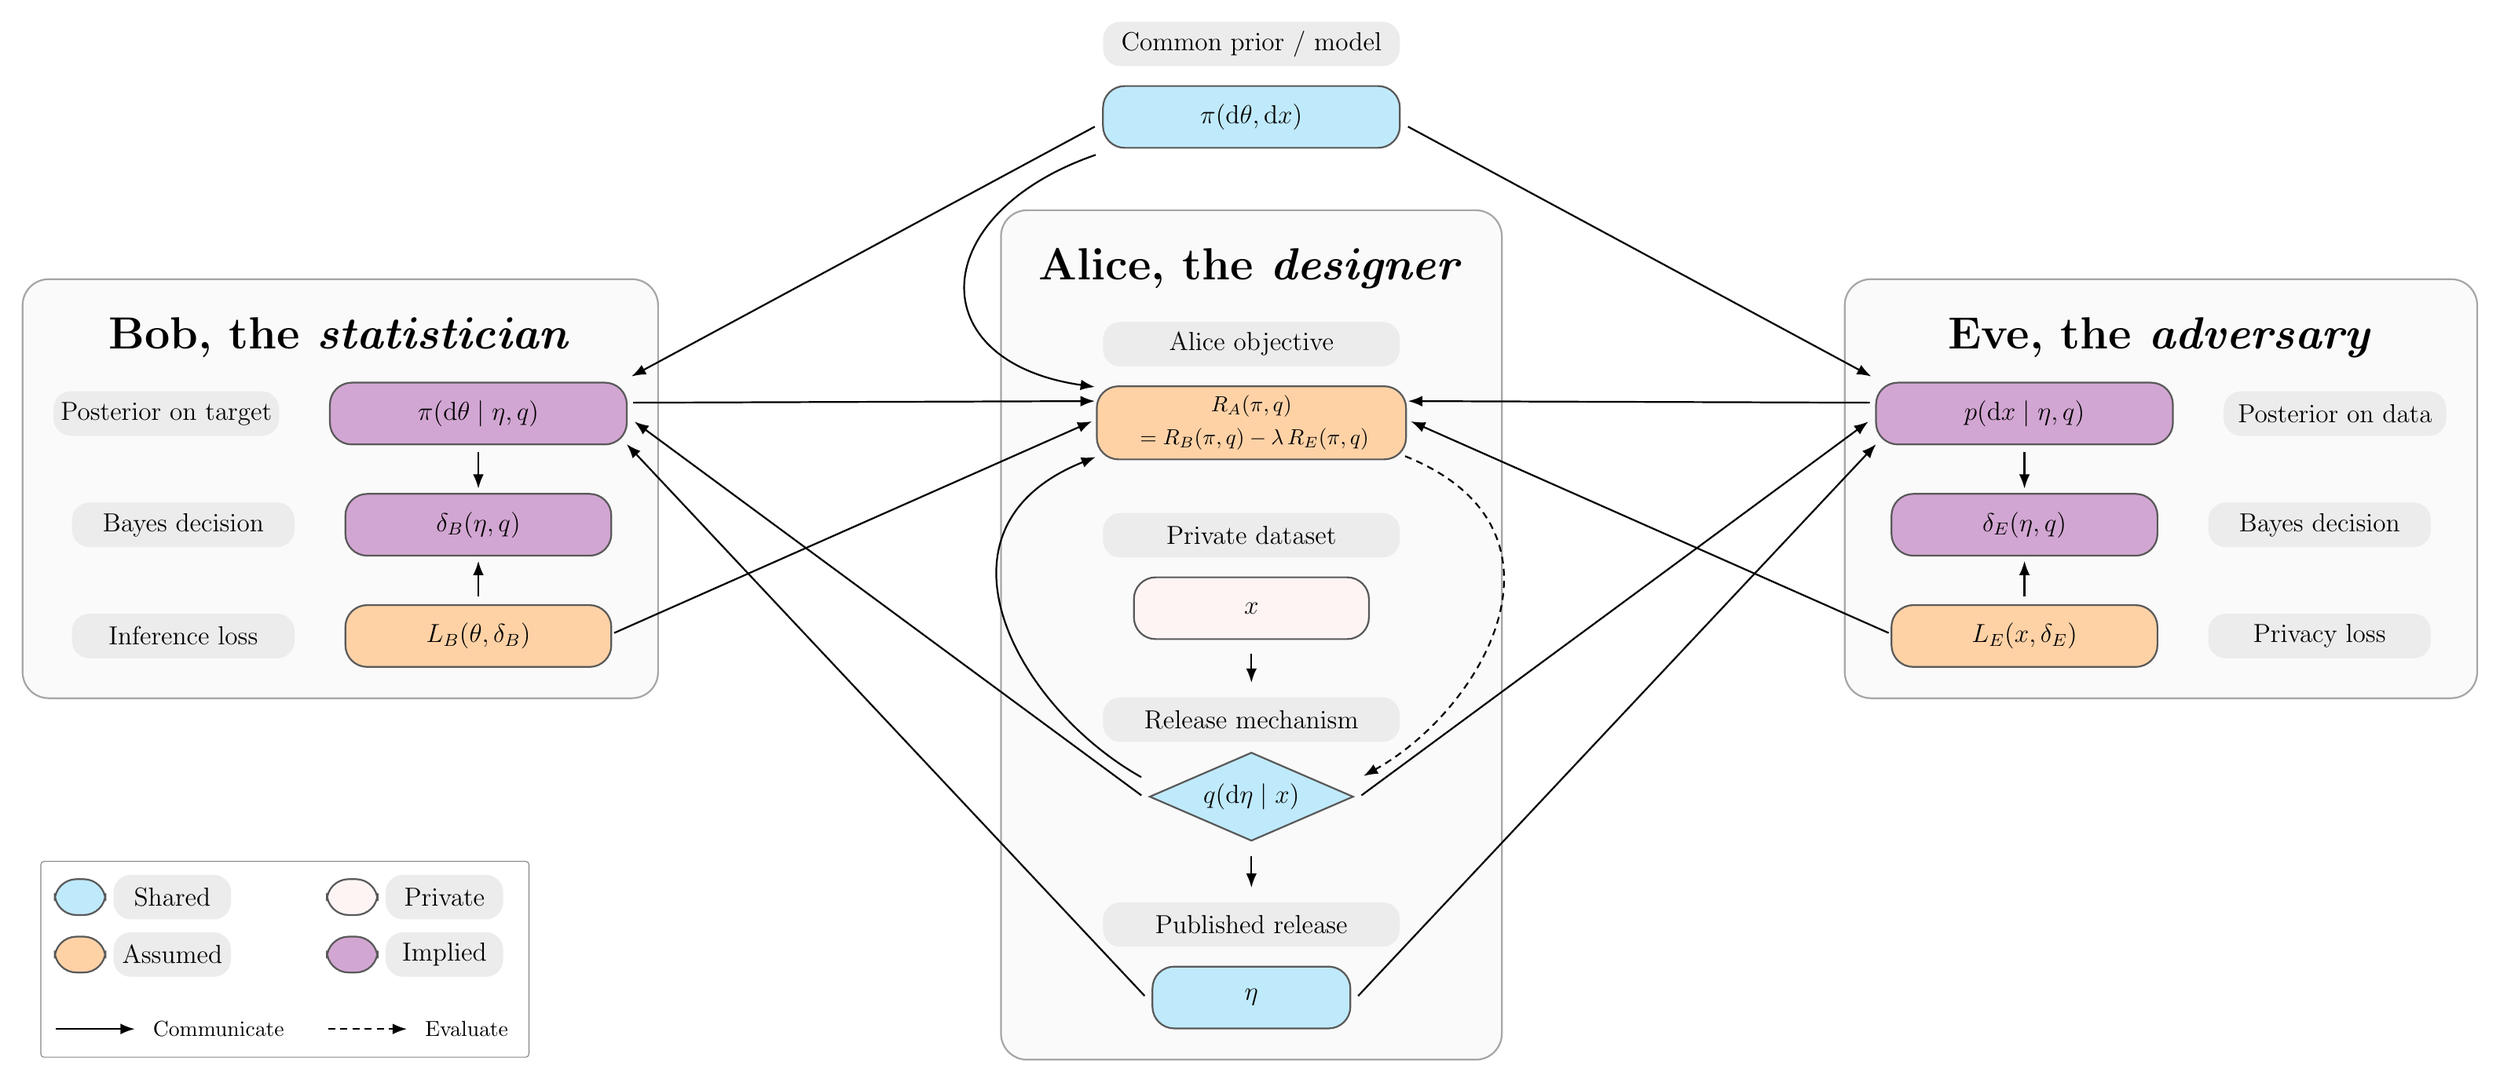
\begin{tikzpicture}[
    >=Latex,
    font=\large,
    box/.style={
        draw=black!65,
        rounded corners=10pt,
        minimum width=4.2cm,
        minimum height=1.0cm,
        align=center,
        thick
    },
    smallbox/.style={
        draw=black!65,
        rounded corners=10pt,
        minimum width=3.5cm,
        minimum height=1.0cm,
        align=center,
        thick
    },
    longbox/.style={
        draw=black!65,
        rounded corners=10pt,
        minimum width=8.5cm,
        minimum height=1.0cm,
        align=center,
        thick
    },
    smalllabel/.style={
        fill=gray!15,
        rounded corners=8pt,
        minimum width=3.6cm,
        minimum height=0.72cm,
        draw=none,
        align=center
    },
    smalllabelwide/.style={
        fill=gray!15,
        rounded corners=8pt,
        minimum width=4.8cm,
        minimum height=0.72cm,
        draw=none,
        align=center
    },
    shared/.style={smallbox, fill=cyan!25},
    private/.style={smallbox, fill=pink!18},
    assumed/.style={box, fill=orange!35},
    implied/.style={box, fill=violet!35},
    mech/.style={
        draw=black!65,
        diamond,
        aspect=2.3,
        fill=cyan!25,
        minimum width=3.0cm,
        minimum height=1.4cm,
        align=center,
        thick
    },
    panel/.style={
        draw=black!35,
        fill=gray!4,
        rounded corners=12pt,
        thick,
        inner sep=14pt
    },
    arr/.style={->, thick, shorten >=2pt, shorten <=1pt},
    arreval/.style={->, thick, dashed, dash pattern=on 3.2pt off 2.4pt, shorten >=2pt, shorten <=1pt},
    % vertical links between stacked Alice boxes (stay in the gap below labels)
    alicevarr/.style={->, thick, shorten >=5pt, shorten <=5pt},
    line/.style={thick}
]

% =========================================================
% MAIN HORIZONTAL ANCHORS
% Make the figure wider by increasing C and R
% =========================================================
\coordinate (L) at (0,0);
\coordinate (C) at (12.5,0);
\coordinate (R) at (25.0,0);

% Useful derived anchors
\coordinate (MidLR) at ($(L)!0.5!(R)$);
% Common vertical axes: column boxes use anchor=center on these $x$ (same $+9$ offset as each anchor)
\coordinate (AliceBoxCenter) at ($(C)+(9,0)$);
\coordinate (BobBoxCenter) at ($(L)+(9,0)$);
\coordinate (EveBoxCenter) at ($(R)+(9,0)$);

% =========================================================
% TITLES (Alice ; Bob/Eve après leurs colonnes — centrés dans le panneau)
% =========================================================
\node[anchor=center, font=\fontsize{22}{26}\selectfont] (titleD) at ($(AliceBoxCenter)+(0,8.5)$)
    {\bfseries Alice, the \emph{designer}};

% =========================================================
% CENTER COLUMN : ALICE
% Prior is intentionally placed in the middle column
% =========================================================
\node[shared, minimum width=4.8cm, anchor=center] (prior) at ($(AliceBoxCenter)+(0,10.95)$)
    {$\pi(\mathrm{d}\theta,\mathrm{d}x)$};
\node[smalllabelwide, anchor=south] (lblprior) at ($(prior.north)+(0,3mm)$)
    {Common prior / model};

\node[assumed, minimum width=5.0cm, minimum height=1.12cm, anchor=center, font=\normalsize] (RA) at ($(AliceBoxCenter)+(0,6.00)$)
    {$\begin{gathered}
        R_A(\pi,q)\\
        {}= R_B(\pi,q)-\lambda\,R_E(\pi,q)
    \end{gathered}$};
\node[smalllabelwide, anchor=south] (lblRA) at ($(RA.north)+(0,3mm)$)
    {Alice objective};

\node[private, minimum width=3.8cm, anchor=center] (x) at ($(AliceBoxCenter)+(0,3.00)$)
    {$x$};
\node[smalllabelwide, anchor=south] (lblx) at ($(x.north)+(0,3mm)$)
    {Private dataset};

\node[mech, anchor=center] (q) at ($(AliceBoxCenter)+(0,-0.05)$)
    {$q(\mathrm{d}\eta\mid x)$};
\node[smalllabelwide, anchor=south] (lblq) at ($(q.north)+(0,1.5mm)$)
    {Release mechanism};

\node[shared, minimum width=3.2cm, anchor=center] (eta) at ($(AliceBoxCenter)+(0,-3.30)$)
    {$\eta$};
\node[smalllabelwide, anchor=south] (lbleta) at ($(eta.north)+(0,3mm)$)
    {Published release};

% $x \to q \to \eta$ : bas de boîte $\to$ haut de la légende ; bas de la légende $\to$ haut de la boîte
\draw[alicevarr] ([yshift=-1.5pt]x.south) -- ([yshift=1.5pt]lblq.north);
\draw[alicevarr] ([yshift=-1.5pt]q.south) -- ([yshift=1.5pt]lbleta.north);

% =========================================================
% LEFT COLUMN : BOB
% =========================================================
\node[implied, minimum width=4.8cm, anchor=center] (postB) at ($(BobBoxCenter)+(0,6.15)$)
    {$\pi(\mathrm{d}\theta\mid \eta,q)$};
\node[smalllabel, anchor=east] (lblpostB) at ($(postB.west)+(-8mm,0)$)
    {Posterior on target};

\node[implied, minimum width=4.3cm, anchor=center] (decB) at ($(BobBoxCenter)+(0,4.35)$)
    {$\delta_B(\eta,q)$};
\node[smalllabel, anchor=east] (lbldecB) at ($(decB.west)+(-8mm,0)$)
    {Bayes decision};

\node[assumed, minimum width=4.3cm, anchor=center] (lossB) at ($(BobBoxCenter)+(0,2.55)$)
    {$L_B(\theta,\delta_B)$};
\node[smalllabel, anchor=east] (lbllossB) at ($(lossB.west)+(-8mm,0)$)
    {Inference loss};

% Titre colonne Bob : au-dessus du postérieur, centré (étiquette ouest $\leftrightarrow$ bord est postérieur)
\coordinate (BobPanelMid) at ($(lblpostB.west)!0.5!(postB.east)$);
\node[anchor=center, font=\fontsize{22}{26}\selectfont] (titleS) at ($(BobPanelMid |- postB.north)+(0,0.72)$)
    {\bfseries Bob, the \emph{statistician}};

% Alice \to Bob : départ flanc gauche du prior $\to$ Bob (xshift pour ne pas coller aux boîtes)
\draw[arr] ([xshift=-2.5pt,yshift=-4pt]prior.west) -- ([yshift=1.5pt]postB.north east);
\draw[arr] ([xshift=-2.5pt]eta.west) -- ([xshift=-1.8pt,yshift=2pt]postB.south east);
% $q\to$ postérieur : flanc du losange ($y$ aligné sur l’ancre ouest / est)
\draw[arr] ([xshift=-2.5pt]q.west) -- ($(postB.east)+(1.5pt,-2.5pt)$);

\draw[arr] ([yshift=-2pt]postB.south) -- (decB.north);
\draw[arr] ([yshift=2.5pt]lossB.north) -- (decB.south);

% =========================================================
% RIGHT COLUMN : EVE
% =========================================================
\node[implied, minimum width=4.8cm, anchor=center] (postE) at ($(EveBoxCenter)+(0,6.15)$)
    {$p(\mathrm{d}x\mid \eta,q)$};
\node[smalllabel, anchor=west] (lblpostE) at ($(postE.east)+(8mm,0)$)
    {Posterior on data};

\node[implied, minimum width=4.3cm, anchor=center] (decE) at ($(EveBoxCenter)+(0,4.35)$)
    {$\delta_E(\eta,q)$};
\node[smalllabel, anchor=west] (lbldecE) at ($(decE.east)+(8mm,0)$)
    {Bayes decision};

\node[assumed, minimum width=4.3cm, anchor=center] (lossE) at ($(EveBoxCenter)+(0,2.55)$)
    {$L_E(x,\delta_E)$};
\node[smalllabel, anchor=west] (lbllossE) at ($(lossE.east)+(8mm,0)$)
    {Privacy loss};

% Titre colonne Eve : symétrique (bord ouest postérieur $\leftrightarrow$ étiquette est)
\coordinate (EvePanelMid) at ($(postE.west)!0.5!(lblpostE.east)$);
\node[anchor=center, font=\fontsize{22}{26}\selectfont] (titleA) at ($(EvePanelMid |- postE.north)+(0,0.72)$)
    {\bfseries Eve, the \emph{adversary}};

% Alice \to Eve : départ flanc droit du prior $\to$ Eve
\draw[arr] ([xshift=2.5pt,yshift=-4pt]prior.east) -- ([yshift=1.5pt]postE.north west);
\draw[arr] ([xshift=2.5pt]eta.east) -- ([xshift=1.8pt,yshift=2pt]postE.south west);
\draw[arr] ([xshift=2.5pt]q.east) -- ($(postE.west)+(-1.5pt,-2.5pt)$);

\draw[arr] ([yshift=-2pt]postE.south) -- (decE.north);
\draw[arr] ([yshift=2.5pt]lossE.north) -- (decE.south);

% =========================================================
% FEED ALICE OBJECTIVE
% =========================================================
% $q\leftrightarrow R_A$ : au niveau $q$, moins de $|dx|$ et plus de $dy$ pour une tangente plus verticale ;
% côté $R_A$, mêmes $\pm\OMdxObj$, $\OMdyObj$ et ancres symétriques (sud-ouest / sud-est).
\def\OMdxMech{2.12}
\def\OMdyMech{1.44}
\def\OMdxObj{2.88}
\def\OMdyObj{1.10}
\def\OMtipX{1.75}
\def\OMtipY{2.25}
% $q\to R_A$ (plein)
\draw[arr]
    ([xshift=-2.5pt,yshift=8.5pt]q.west)
    .. controls ($(q.west)+(-\OMdxMech,\OMdyMech)$) and ($(RA.south west)+(-\OMdxObj,-\OMdyObj)$)
    .. ([xshift=\OMtipX pt,yshift=\OMtipY pt]RA.south west);

% $R_A \to q$ (tirets)
\draw[arreval]
    ([xshift=-\OMtipX pt,yshift=\OMtipY pt]RA.south east)
    .. controls ($(RA.south east)+(\OMdxObj,-\OMdyObj)$) and ($(q.east)+(\OMdxMech,\OMdyMech)$)
    .. ([xshift=2.5pt,yshift=8.5pt]q.east);

% prior $\to R_A$ : départ bas-gauche du prior ; arrive nord-ouest de $R_A$
\draw[arr]
    ([xshift=-2pt,yshift=-2.5pt]prior.south west)
    .. controls ($(prior.south west)+(-2.85,-1.05)$) and ($(RA.north west)+(-2.85,0.38)$)
    .. ([xshift=1.5pt,yshift=-1pt]RA.north west);

% pertes $\to R_A$ : milieu des flancs gauche et droit (pas les coins bas liés au mécanisme)
\draw[arr] ([yshift=1pt]lossB.east) -- ([yshift=1.5pt]RA.west);
\draw[arr] ([yshift=1pt]lossE.west) -- ([yshift=1.5pt]RA.east);

% postérieurs $\to R_A$ (au-dessus des flèches de perte ; mêmes $\pm1.5\,\mathrm{pt}$ que $q\to$postérieurs)
\draw[arr] ([xshift=1.5pt,yshift=5pt]postB.east) -- ([xshift=1.5pt,yshift=10pt]RA.west);
\draw[arr] ([xshift=-1.5pt,yshift=5pt]postE.west) -- ([xshift=-1.5pt,yshift=10pt]RA.east);

% =========================================================
% PANELS (behind nodes and arrows)
% =========================================================
\begin{scope}[on background layer]
    \node[panel, fit=(titleS)(lblpostB)(postB)(lbldecB)(decB)(lbllossB)(lossB)] (panelS) {};
    \node[panel, fit=(titleD)(lblx)(x)(lblq)(q)(lbleta)(eta)(lblRA)(RA)] (panelD) {};
    \node[panel, fit=(titleA)(lblpostE)(postE)(lbldecE)(decE)(lbllossE)(lossE)] (panelA) {};
\end{scope}

% =========================================================
% LEGEND : bas = bas du panneau Alice (panelD), gauche = gauche du panneau Bob (panelS)
% Grille $3$ lignes $\times$ $2$ colonnes (pastilles + flèches)
% =========================================================
\def\LegLeftX{0.32}
\def\LegRightX{4.72}
\def\LegYOne{2.05}
\def\LegYTwo{1.12}
\def\LegYThr{0.22}
\def\LegBaseln{2.5pt}% profondeur approx. du texte (rangée flèches) pour aligner legframe.sud sur panelD.sud
\coordinate (LegSW) at ($ (panelS.west |- panelD.south) + (-\LegLeftX + 6pt, -\LegYThr + 6pt + \LegBaseln) $);

% Ligne 1 : Shared [ Private
\node[shared, minimum width=0.82cm, minimum height=0.58cm, anchor=south west] (leg1)
    at ($(LegSW)+(\LegLeftX,\LegYOne)$) {};
\node[smalllabel, minimum width=1.9cm, anchor=west] (leg1t) at ($(leg1.east)+(0.11,0)$) {Shared};
\node[private, minimum width=0.82cm, minimum height=0.58cm, anchor=south west] (leg2)
    at ($(LegSW)+(\LegRightX,\LegYOne)$) {};
\node[smalllabel, minimum width=1.9cm, anchor=west] (leg2t) at ($(leg2.east)+(0.11,0)$) {Private};

% Ligne 2 : Assumed | Implied
\node[assumed, minimum width=0.82cm, minimum height=0.58cm, anchor=south west] (leg3)
    at ($(LegSW)+(\LegLeftX,\LegYTwo)$) {};
\node[smalllabel, minimum width=1.9cm, anchor=west] (leg3t) at ($(leg3.east)+(0.11,0)$) {Assumed};
\node[implied, minimum width=0.82cm, minimum height=0.58cm, anchor=south west] (leg4)
    at ($(LegSW)+(\LegRightX,\LegYTwo)$) {};
\node[smalllabel, minimum width=1.9cm, anchor=west] (leg4t) at ($(leg4.east)+(0.11,0)$) {Implied};

% Ligne 3 : Communicate | Evaluate
\node[coordinate] (legsolidL) at ($(LegSW)+(\LegLeftX,\LegYThr)$) {};
\node[coordinate] (legsolidR) at ($(LegSW)+(\LegLeftX+1.38,\LegYThr)$) {};
\draw[arr] (legsolidL) -- (legsolidR);
\node[anchor=west, font=\normalsize] (legTxtComm) at ($(legsolidR)+(0.1,0)$) {Communicate};

\node[coordinate] (legdashL) at ($(LegSW)+(\LegRightX,\LegYThr)$) {};
\node[coordinate] (legdashR) at ($(LegSW)+(\LegRightX+1.38,\LegYThr)$) {};
\draw[arreval] (legdashL) -- (legdashR);
\node[anchor=west, font=\normalsize] (legTxtEval) at ($(legdashR)+(0.1,0)$) {Evaluate};

\begin{scope}[on background layer]
    \node[draw=black!48, fill=white, rounded corners=1.5pt, inner sep=6pt,
          fit=(leg1)(leg1t)(leg2)(leg2t)(leg3)(leg3t)(leg4)(leg4t)
              (legsolidL)(legsolidR)(legTxtComm)(legdashL)(legdashR)(legTxtEval)] (legframe) {};
\end{scope}

\end{tikzpicture}

\end{document}